% Section content template for individual Educative lessons
% This file contains the actual content for a specific section
% Generated from Educative API section content

% Section: Detailed Design of Instagram
% Section ID: 6638179708305408
% Section Slug: detailed-design-of-instagram
% Generated: 2025-12-08T13:40:33.890156

\subsection{Add more components}\label{z6UDGx5qb2pmxRoEX40xj}
\\
Let's add a few more components to our design:

\begin{itemize}
\item
\protect\phantomsection\label{qGR6WRJ_l7ZBnLe_QwIBW}
\href{https://www.educative.io/courses/grokking-the-system-design-interview/introduction-to-load-balancers}{\textbf{Load balancer}}: To balance the load of the requests from the end users.
\item
\protect\phantomsection\label{nkAoNtUCXbugwzLICAKJV}
\textbf{Application servers}: To host our service to the end users.
\item
\protect\phantomsection\label{fxtJDJ-hGYvHcuzdw6mI4}
\href{https://www.educative.io/courses/grokking-the-system-design-interview/introduction-to-databases}{\textbf{Relational database}}: To store our data.
\item
\protect\phantomsection\label{LVqs2Cdfuh4BWvaugIPva}
\href{https://www.educative.io/courses/grokking-the-system-design-interview/system-design-a-blob-store}{\textbf{Blob storage}}: To store the photos and videos uploaded by the users.
\end{itemize}

\begin{figure}[htbp]
 \centering
 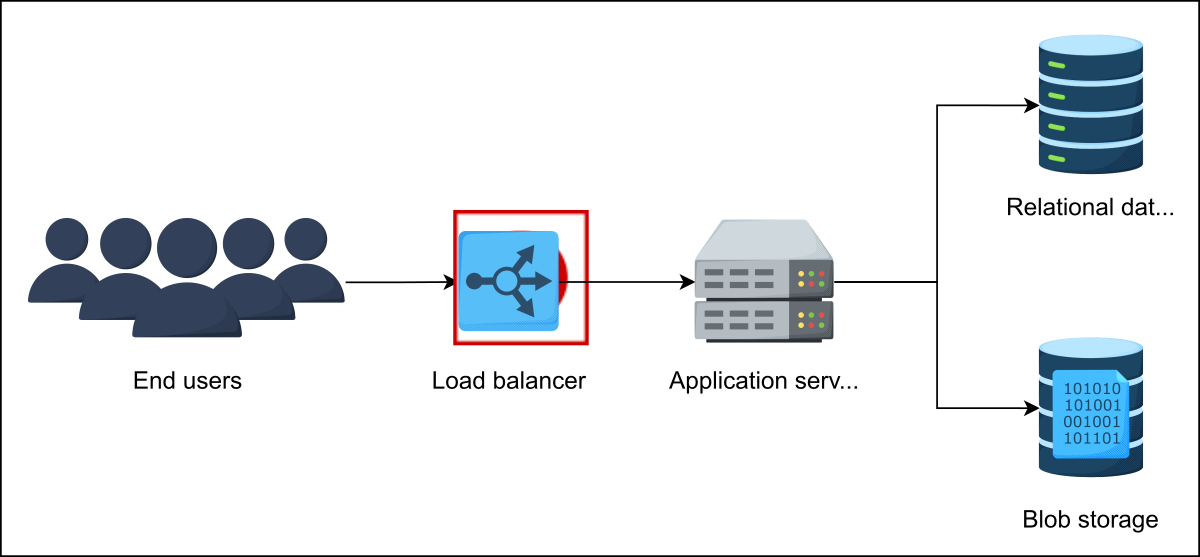
\includegraphics[width=0.5\textwidth]{Images/chapter_33/section_6638179708305408/6647922215485440.png}
 \caption{Adding components to design}
\end{figure}

\subsection{Upload, view, and search a photo}\label{23KhUH1yHZnZ8_SRY9Ror}
\\
The client requests to upload the photo, load balancer passes the request to any of the application servers, which adds an entry to the database. An update that the photo is stored successfully is sent to the user. If an error is encountered, the user is communicated about it as well.
\\
The photo viewing process is also similar to the above-mentioned flow. The client requests to view a photo, and an appropriate photo that matches the request is fetched from the database and shown to the user. The client can also provide a keyword to search for a specific image.
\\
The read requests are more than write requests and it takes time to upload the content in the system. It is efficient if we separate the write (uploads) and read services. The multiple services operated by many servers handle the relevant requests. The read service performs the tasks of fetching the required content for the user, while the write service helps upload content to the system.
\\
We also need to cache the data to handle millions of reads. It improves the user experience by making the fetching process fast. We 'll also opt for lazy loading(Lazy loading contributes to efficiency in the program's operation. It is ideal in use cases where network content is accessed and initialization times are to be kept at a minimum, such as in the case of web pages. For example, deferring the loading of images on a web page until they are needed can make the initial display of the web page faster. Source
: Wikipedia), which minimizes the client's waiting time. It allows us to load the content when the user scrolls and therefore save the bandwidth and focus on loading the content the user is currently viewing. It improves the latency to view or search a particular photo or video on Instagram.
\\
The updated design is as follows:

\begin{figure}[htbp]
 \centering
 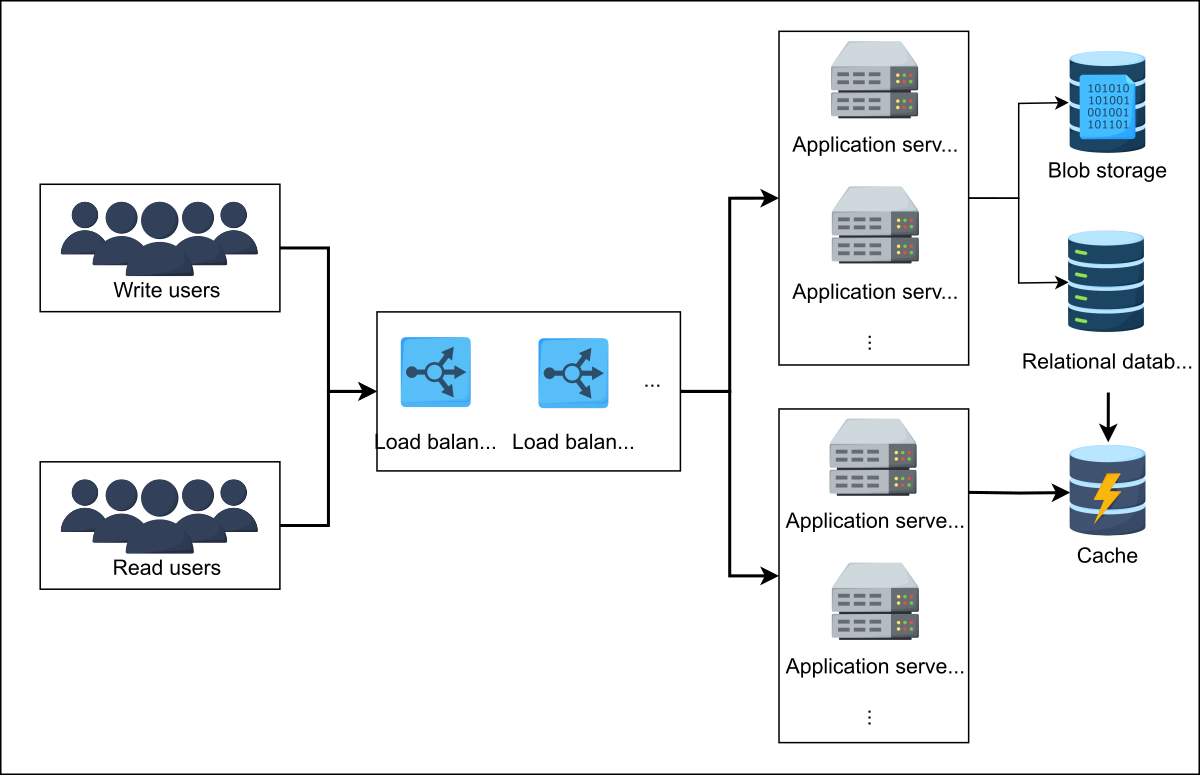
\includegraphics[width=0.5\textwidth]{Images/chapter_33/section_6638179708305408/6205852405334016.png}
 \caption{Various operations on photos}
\end{figure}

\subsection{Generate a timeline}\label{weFVC5QN-QIl-7pk0O04x}
\\
Now our task is to generate a user-specific timeline. Let 's explore various approaches and the advantages and disadvantages to opt for the appropriate strategy.

\subsubsection{The pull approach}\label{5rdbq0WDLMJyxoVI7Qzat}
\\
When a user opens their Instagram, we send a request for timeline generation. First , we fetch the list of people the user follows, get the photos they recently posted, store them in queues, and display them to the user. But this approach is slow to respond as we generate a timeline every time the user opens Instagram.\\
\strut \\
We can substantially reduce user-perceived latency by generating the timeline offline. For example, we define a service that fetches the relevant data for the user before, and as the person opens Instagram, it displays the timeline. This decreases the latency rate to show the timeline. Let 's take a look at the slides below to understand the problem and its solution.

\begin{figure}[htbp]
 \centering
 \begin{subfigure}[b]{0.48\textwidth}
 \centering
 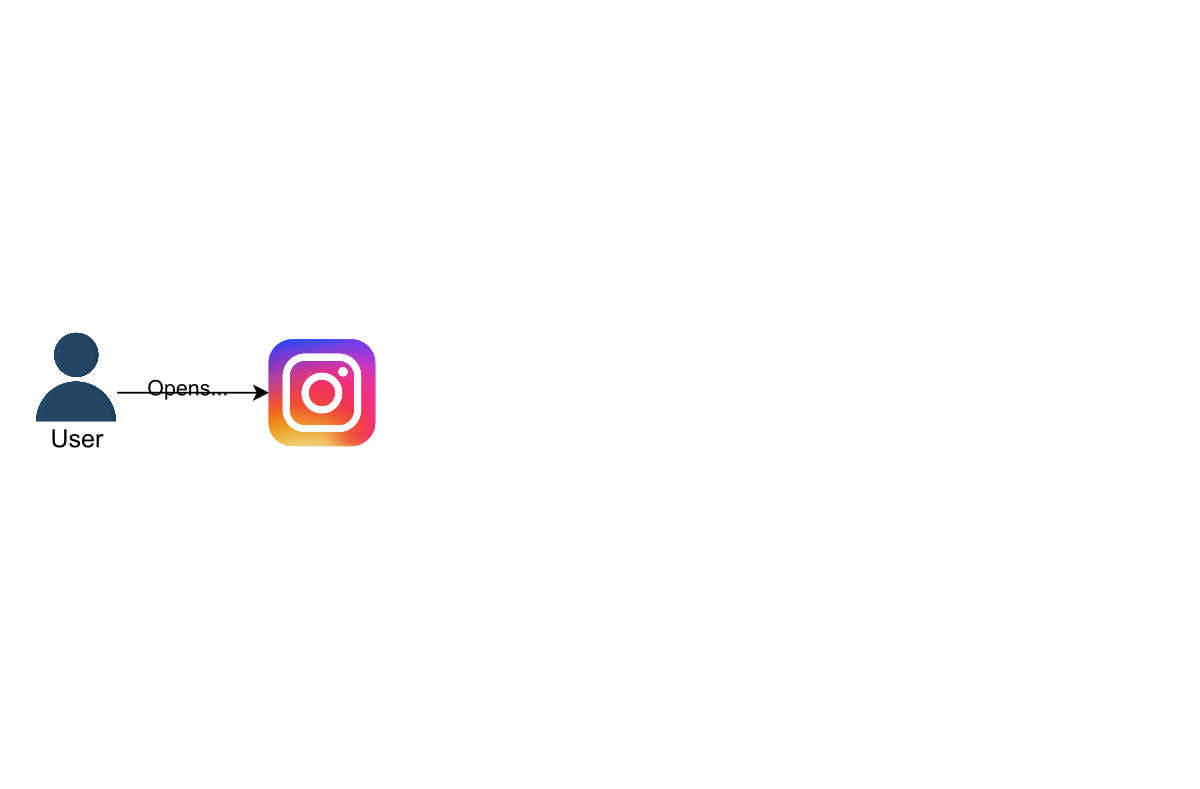
\includegraphics[width=\textwidth]{Images/chapter_33/section_6638179708305408/6247946513547264.png}
 \caption{A user opens Instagram}
 \end{subfigure}
 \hfill
 \begin{subfigure}[b]{0.48\textwidth}
 \centering
 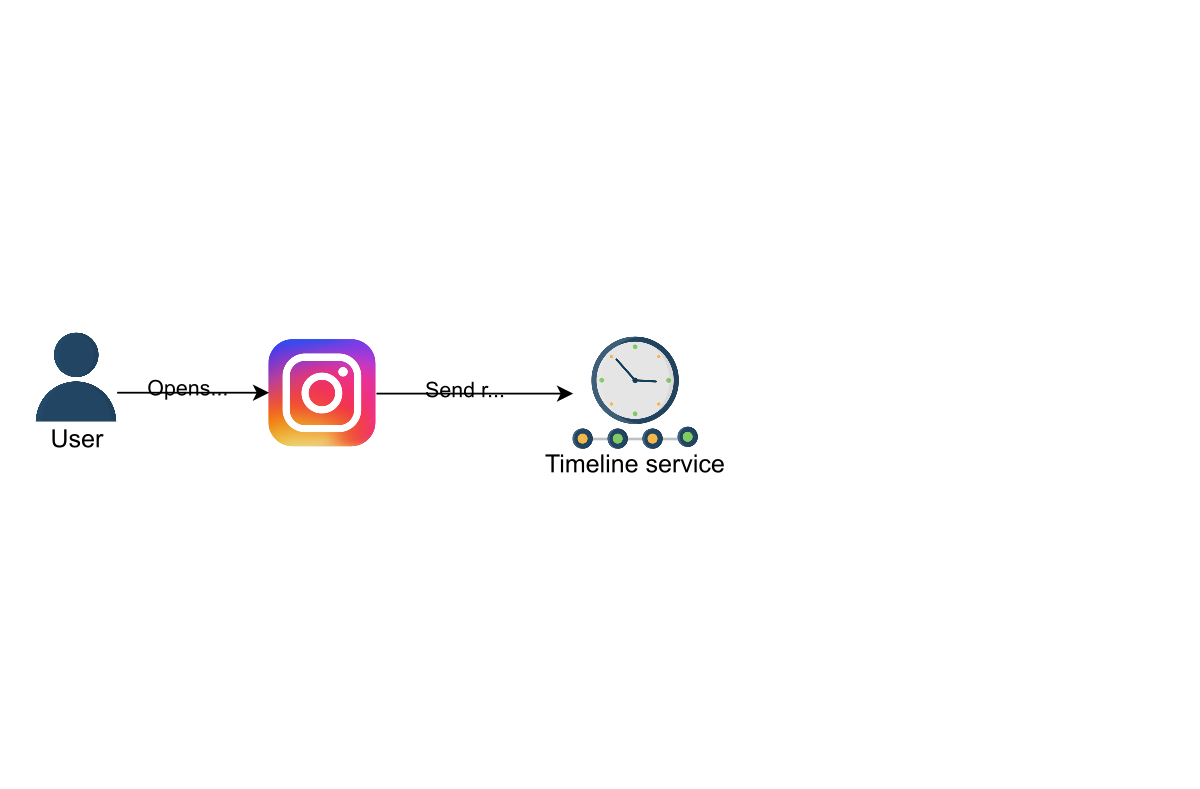
\includegraphics[width=\textwidth]{Images/chapter_33/section_6638179708305408/5503694347173888.png}
 \caption{A request to generate a timeline is sent to the timeline service}
 \end{subfigure}
\end{figure}

\begin{figure}[htbp]
 \centering
 \begin{subfigure}[b]{0.48\textwidth}
 \centering
 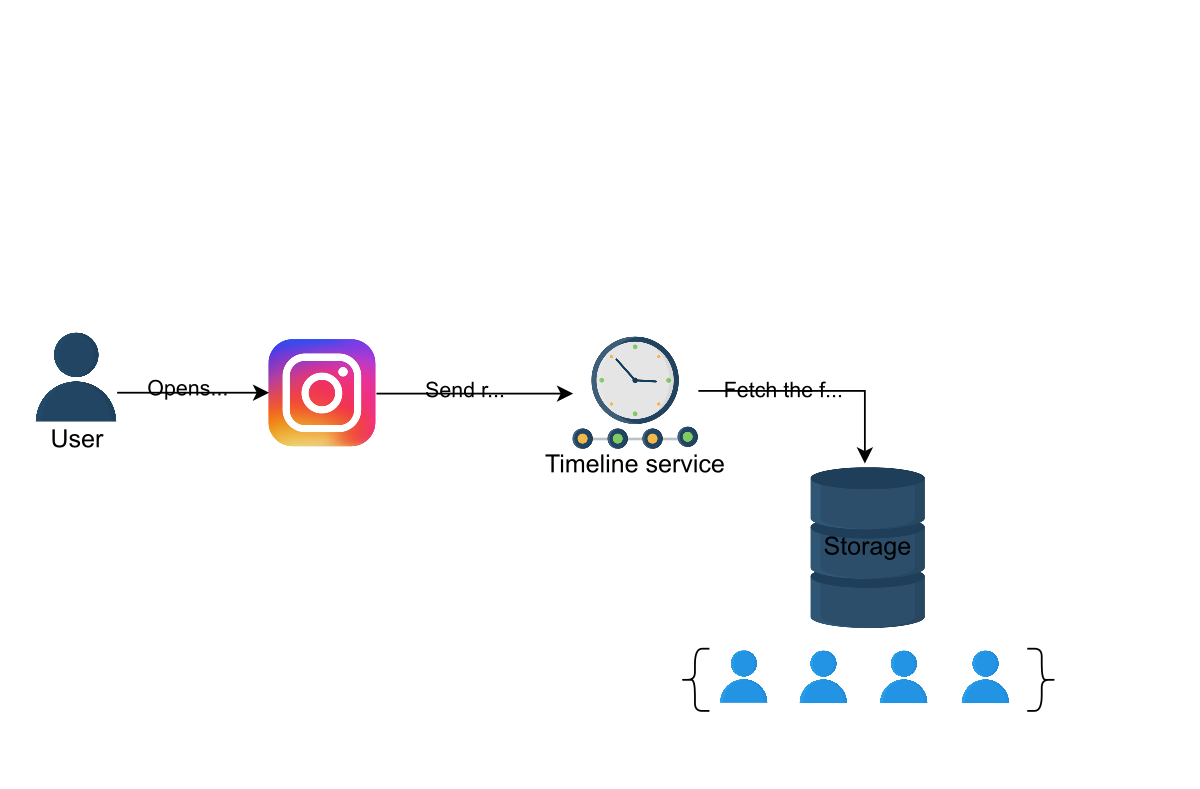
\includegraphics[width=\textwidth]{Images/chapter_33/section_6638179708305408/6463950283866112.png}
 \caption{The timeline service fetches the list of followers for that user from the storage}
 \end{subfigure}
 \hfill
 \begin{subfigure}[b]{0.48\textwidth}
 \centering
 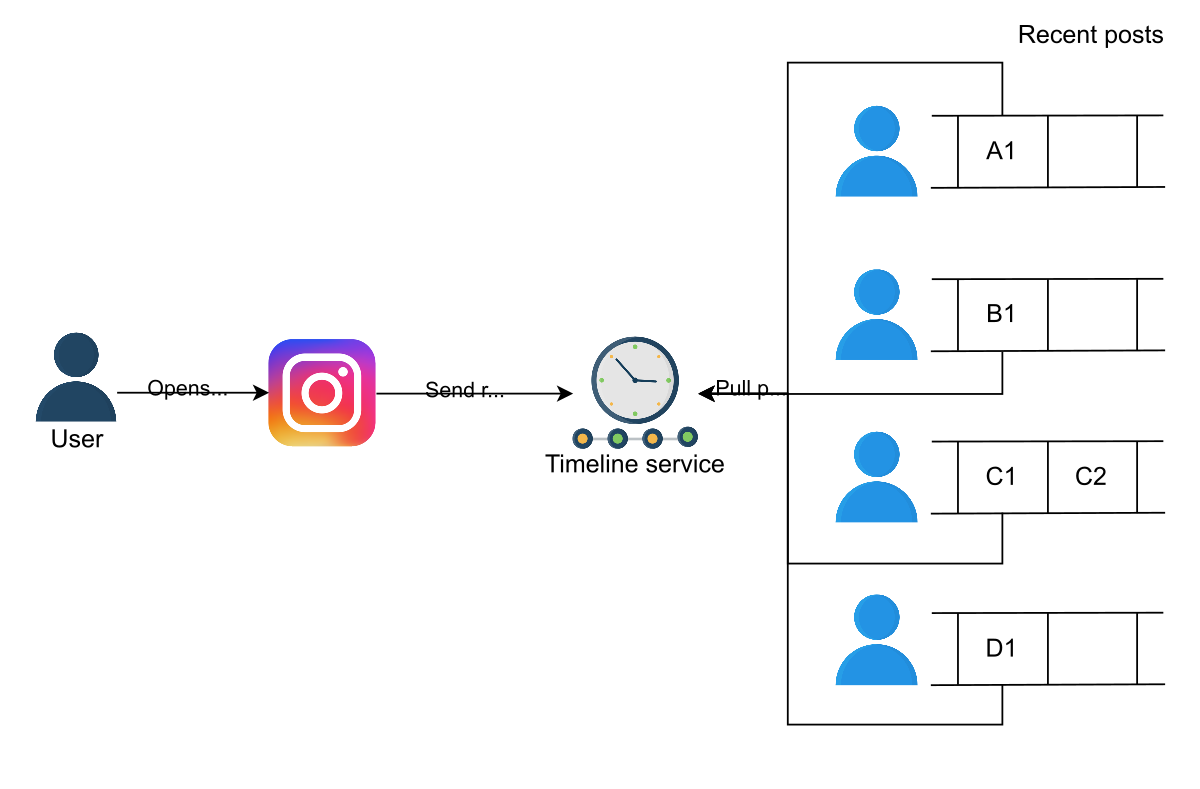
\includegraphics[width=\textwidth]{Images/chapter_33/section_6638179708305408/5805651653820416.png}
 \caption{The timeline service fetches the recent posts of the followers}
 \end{subfigure}
\end{figure}

\begin{figure}[htbp]
 \centering
 \begin{subfigure}[b]{0.48\textwidth}
 \centering
 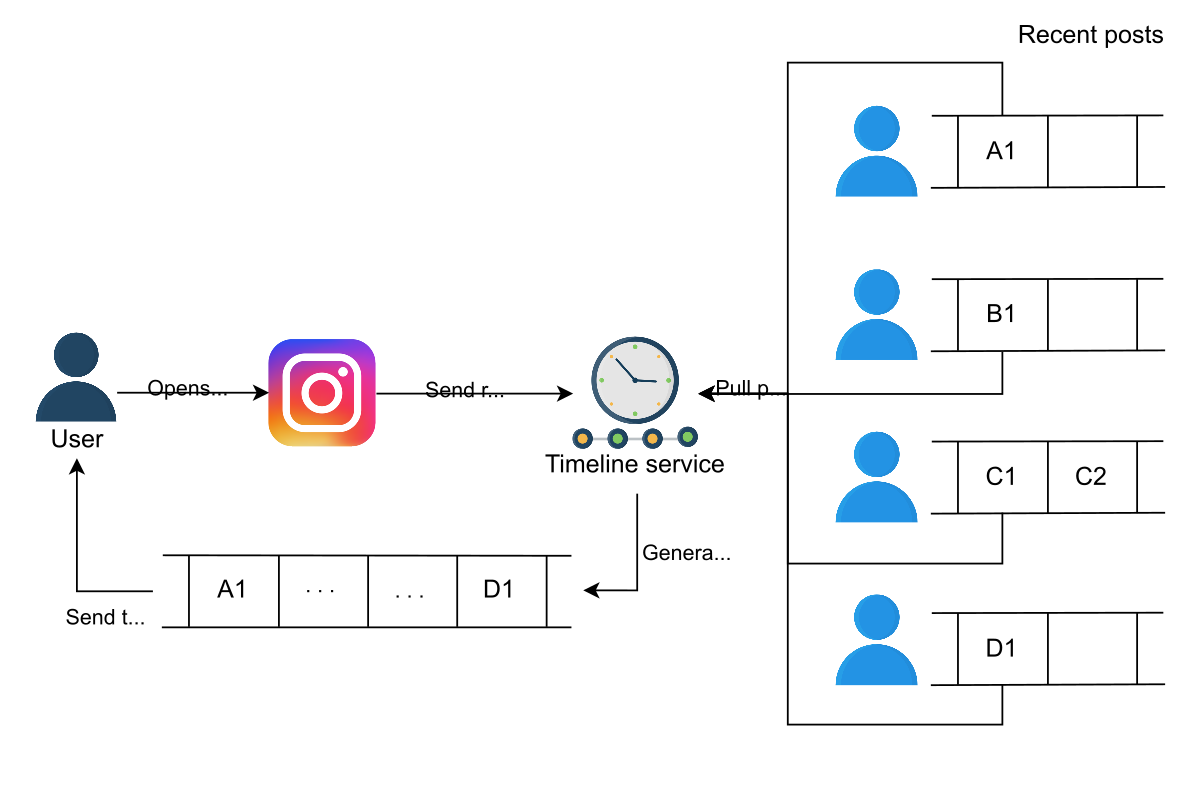
\includegraphics[width=\textwidth]{Images/chapter_33/section_6638179708305408/4854745760268288.png}
 \caption{Display the fetched photos on the user's timeline}
 \end{subfigure}
\end{figure}

\begin{quote}
\textbf{Quiz:}
\textbf{Question 1:} What are the shortcomings of the pull approach?
\textbf{Answer:} Instagram is a read-heavy system. Many people don't post any photos and instead just view others' posts. So, the calls we make to fetch the recent posts from every follower will usually return nothing. Hence, we should keep in mind that it is not a write-heavy system and should develop a possible solution to cater to it.
\end{quote}

\subsubsection{The push approach}\label{0CWF4j7Bb9ZSbk4niXrq-}
\\
In a \textbf{push approach}, every user is responsible for pushing the content they posted to the people's timelines who are following them. In the previous approach, we pulled the post from each follower, but in the current approach, we push the post to each follower.
\\
Now we only need to fetch the data that is pushed towards that particular user to generate the timeline. The push approach has stopped a lot of requests that return empty results when followed users have no post in a specified time.

\begin{figure}[htbp]
 \centering
 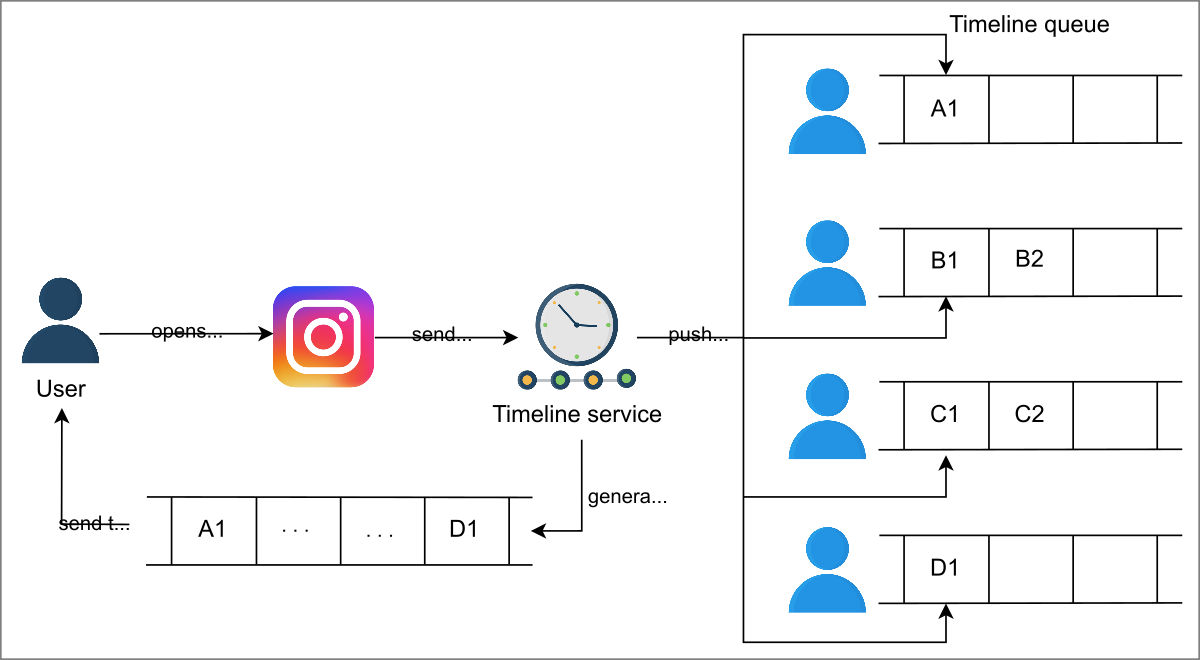
\includegraphics[width=0.5\textwidth]{Images/chapter_33/section_6638179708305408/6745267059818496.png}
 \caption{Push-based approach}
\end{figure}

\begin{quote}
\textbf{Quiz:}
\textbf{Question 1:} What are the shortcomings of the push approach?
\textbf{Answer:} Consider an account that belongs to a celebrity, like Cristiano Ronaldo,

who has over 400 million followers. So if he posts a photo or a video, we will push the links of the photo/video to 400 million+ users, which is inefficient.
\end{quote}

\subsubsection{Hybrid approach}\label{Oj_6qY6ID0j3tNb9eUjLb}
\\
Let's split our users into two categories:

\begin{itemize}
\item
\protect\phantomsection\label{6_6uMR1IJG1aUWXlbEBri}
\textbf{Push-based users}: The users who have a followers count of hundreds or thousands.
\item
\protect\phantomsection\label{Yv-SDoHNJC1AmnF5Ko3Q7}
\textbf{Pull-based users}: The users who are celebrities and have followers count of a hundred thousand or millions.
\end{itemize}
\\
The timeline service pulls the data from pull-based followers and adds it to the user's timeline. The push-based users push their posts to the timeline service of their followers so the timeline service can add to the user's timeline.

\begin{figure}[htbp]
 \centering
 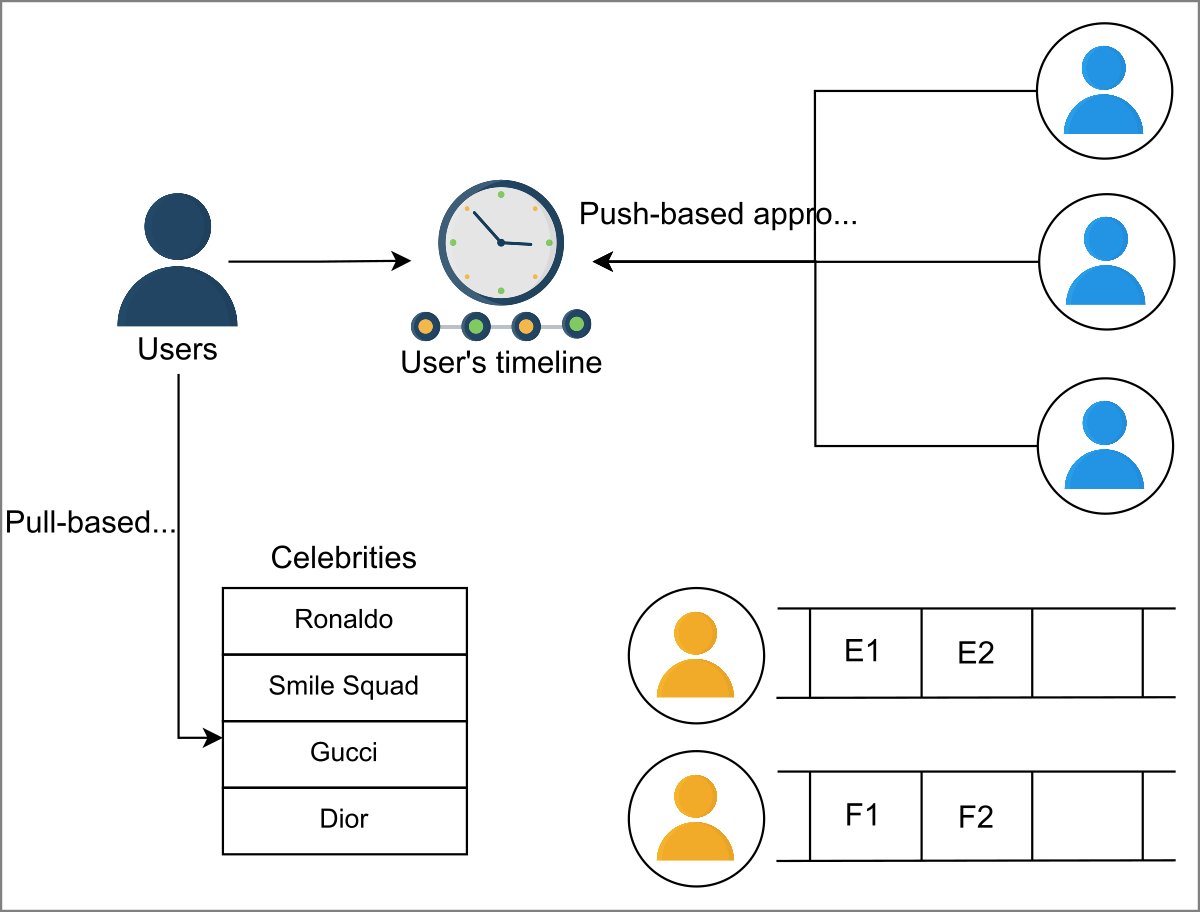
\includegraphics[width=0.5\textwidth]{Images/chapter_33/section_6638179708305408/4976013826326528.png}
 \caption{Hybrid approach}
\end{figure}

We have used the method which generates the timeline, but where do we store the timeline? We store a user's timeline against a \texttt{userID} in a key-value store. Upon request, we fetch the data from the key-value store and show it to the user. The key is \texttt{userID}, while the value is timeline content (links to photos and videos). Because the storage size of the value is often limited to a few MegaBytes, we can store the timeline data in a blob and put the link to the blob in the value of the key as we approach the size limit.
\\
We can add a new feature called story to our Instagram. In the story feature, the users can add a photo that stays available for others to view for 24 hours only. We can do this by maintaining an option in the table where we can store a story's duration. We can set it to 24 hours, and the \href{https://www.educative.io/courses/grokking-the-system-design-interview/system-design-the-distributed-task-scheduler}{task scheduler} deletes the entries whose time exceeds the 24 hours limit.

\subsection{Finalized design}\label{h5PCahP-7aoCSR5b64Bn2}
\\
We'll also use \textbf{CDN (content delivery network)} in our design. We can keep images and videos of celebrities in CDN which make it easier for the followers to fetch them. The load balancer first routes the read request to the nearest CDN, if the requested content is not available there, then it forwards the request to the particular read application server (see the ``\href{https://www.educative.io/courses/grokking-the-system-design-interview/introduction-to-load-balancers}{load balancing chapter}'' for the details). The CDN helps our system to be available to millions of concurrent users and minimizes latency.
\\
The final design is given below:

\begin{figure}[htbp]
 \centering
 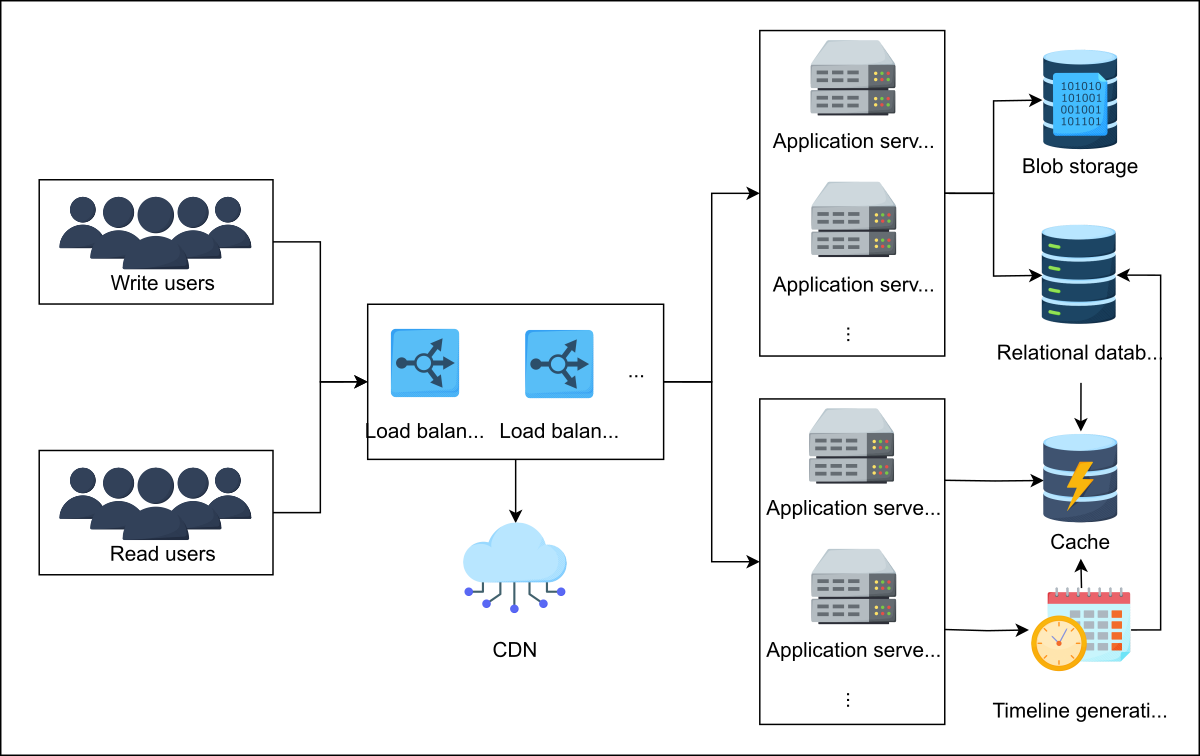
\includegraphics[width=0.5\textwidth]{Images/chapter_33/section_6638179708305408/4838441068396544.png}
 \caption{The final design of Instagram}
\end{figure}

\begin{quote}
\textbf{Quiz:}
\textbf{Question 1:} How can we count millions of interactions (like or view) on a celebrity post?
\textbf{Answer:} We can use {[} sharded counters{]}(https://www.educative.io/courses/grokking-the-system-design-interview/system-design-the-sharded-counters)

to count the number of multiple interactions for a particular user. Each counter has a number of shards distributed across various edge servers to reduce the load on the application server and latency. Users nearest to the edge server get the updated count frequently on a specific post compared to those in distant regions.
\end{quote}

\subsection{Requirements compliance}\label{DuDD21elb6-TCAOqjpFjC}
\\
Let's evaluate the Instagram design with respect to its non-functional requirements:

\begin{itemize}
\item
\protect\phantomsection\label{iy_ft0cWCoLIkG6Wy4aue}
\textbf{Scalability}: We can add more servers to the application service layers to make the scalability better and handle numerous requests from the clients. We can also increase the number of databases to store the growing users' data.
\item
\protect\phantomsection\label{v6BqPOU2XFRtWnGYVyHYR}
\textbf{Latency}: The use of cache and CDNs has reduced the content fetching time.
\item
\protect\phantomsection\label{Ia_bHvAit5oFoIi3Ba-0C}
\textbf{Availability}: We have made the system available to the users by using the storage and databases that are replicated across the globe.
\item
\protect\phantomsection\label{VAFACd52Zi9W-RUDpYqkx}
\textbf{Durability:} We have persistent storage that maintains the backup of the data, so any uploaded content (photos and videos) never gets lost.
\item
\protect\phantomsection\label{F7w4q43Le4SuFbY8iFVTZ}
\textbf{Consistency}: We have used storage like blob stores and databases to keep our data consistent globally.
\item
\protect\phantomsection\label{NISC7rh16wiZwG73deARR}
\textbf{Reliability}: Our databases handle \href{https://www.educative.io/courses/grokking-the-system-design-interview/data-replication}{replication} and redundancy, so our system stays reliable and data is not lost. The load balancing layer routes requests around failed servers.
\end{itemize}

\subsection{Conclusion}\label{J2GKQbaIkAYXwZLqrVomR}
\\
This design problem highlights that we can provide major services by connecting our building blocks appropriately. The scalable and fault-tolerant building blocks enable us to concentrate on use-case-specific issues (such as the efficient formation of timelines).

% End of section content